\documentclass[14pt]{extreport}
\usepackage[utf8]{vietnam}
%\usepackage{type1cm}
\usepackage[left=3.50cm, right=2.00cm, top=3.50cm, bottom=3.00cm]{geometry}
%\usepackage[left=3.0cm, right=1.50cm, top=3.00cm, bottom=2.50cm]{geometry}
\usepackage{graphicx}
\usepackage{mathrsfs} 
\usepackage{amsfonts}
\usepackage{longtable}
\usepackage[intlimits]{amsmath}
\usepackage{array}
\usepackage{amsxtra,amssymb,latexsym,amscd,amsthm}
\newtheorem{theorem}{\MakeUppercase{K}ết quả}[section]
% khoảng cách dòng 1.5 lines (như trong MS Word)
\renewcommand{\baselinestretch}{1.5}

%——————–
\begin{document}
%tao khung
\newcommand{\Khung}[2]{
\begin{tabular}{|l|}
\hline\rule[-2ex]{0pt}{5.5ex}
\parbox{#1}{#2}\\
\hline
\end{tabular}
}

\Khung{.92\textwidth}{

\begin{center}
\normalsize
\textbf{TRƯỜNG ĐẠI HỌC BÁCH KHOA HÀ NỘI}\\
\normalsize
\textbf{VIỆN TOÁN ỨNG DỤNG VÀ TIN HỌC}\\
\textbf{------------------------------------------------------}\\[0.4cm]

\includegraphics[scale=.8]{logobkdentrang}\\[1.2cm]
\textbf{{ BÀI TẬP LỚN:}}\\
\textbf{{\large ỨNG DỤNG HỌC TĂNG CƯỜNG VÀO}}\\
\textbf{{\largeĐẦU TƯ CHỨNG KHOÁN}}\\
\end{center}
\begin{flushleft}
\vspace{1.3cm}
\hspace{1.5cm} \textbf{ Giáng viên hướng dẫn:{ TS. Nguyễn Thị Ngọc Anh }}\\[0.2cm]
\hspace{1.5cm} \textbf{ Nhóm Sinh viên thực hiện:}\\[0.2cm]
\hspace{7.4cm}\textbf{ Vũ Thị Ngọc}\\[0.2cm]
\hspace{7.4cm}\textbf{ Trịnh Hoàng Đức}\\[0.2cm]
\hspace{7.4cm}\textbf{ Đặng Đình Trung}\\[0.2cm]
\hspace{1.5cm} \textbf{ Lớp:\hspace{4.5cm}{ KSTN Toán Tin K60}}\\
\end{flushleft}

\begin{center}
\textbf{{\small HÀ NỘI - 06/2018}}\\
\end{center}
 }
\thispagestyle{empty}
\newpage

\tableofcontents
\newpage

%\listoffigures

\newpage
\chapter{Giới thiệu bài toán}

Ngày nay, việc đầu tư chứng khoán là lĩnh vực đầu tư phát triển rất mạnh, thu hút sự quan tâm của không ít các nhà đầu tư trên khắp thế giới. Nhà đầu tư tốt sẽ thu được lợi nhuận kể cả khi giá cổ phiếu có chiều hướng tăng hoặc giảm. Cụ thể:

$\quad \bullet$ Khi cổ phiếu đang có xu hướng tăng, nhà đầu tư sẽ mua cổ phiếu đó trước khi giá tiếp tục tăng và bán trước khi giá sẽ giảm

$\quad \bullet$ Khi cổ phiếu đang có xu hướng giảm, nhà đầu tư sẽ đi vay cổ phiếu và lập tức bán đi. Đợi khi giá cổ phiếu giảm đến một mức nào đó, nhà đầu tư sẽ đi mua lại đủ cổ phiếu và trả cho người đã cho vay

Chiến lược đầu tư rất thông minh phải không? Tuy nhiên vấn đề ở đây là ta biết khi nào giá cổ phiếu đang có xu hướng tăng và khi nào giảm.
\\ 

Dựa trên suy nghĩ rằng giá cổ phiếu thay đổi là có quy luật, người ta xây dựng một cách tiếp cận tương đối mới với giao dịch tài chính là sử dụng thuật toán học máy để dự đoán giá cổ phiếu tăng hoặc giảm trước khi nó xảy ra.

Trong bài này, nhóm em xin trình bày một cách tiếp cận như vậy với phương pháp học tăng cường và sử dụng ý tưởng cốt lõi để tối ưu là phương pháp hướng tăng Gradient. Cụ thể:

$\quad \bullet$ \textit{Chương 2: Các khái niệm cơ bản về học tăng cường và phương pháp hướng tăng Gradient}

$\quad \bullet$ \textit{Chương 3: Cách ứng dụng vào đầu tư chứng khoán}

$\quad \bullet$ \textit{Chương 4: Kết luận và một số kết quả được nhóm rút ra trong quá trình làm}

\chapter{Phương pháp}
\section{Giới thiệu}

 Trong ngành khoa học máy tính, học tăng cường (Reinforcement Learning) là một lĩnh vực con của học máy (Machine Learning), nghiên cứu cách thức một tác tử (agent) trong một môi tường nên chọn thực hiện các hành động nào để có được phần thưởng có giá trị lớn nhất về lâu về dài. Các thuật toán học tăng cường cố gắng tìm một chiến lược ánh xạ từ không gian trạng thái tới không gian hành động mà agent nên chọn trong các trạng thái đó.
 
 
\section{Quá trình quyết định Markov}

 Quá trình quyết định Markov (Markov Decision Processes, viết tắt là MDP) cung cấp một nền tảng toán học cho việc mô hình hóa việc ra quyết định trong các tình huống mà kết quả là một phần ngẫu nhiên, một phần dưới sự điều khiển của một người ra quyết định. MDP rất hữu dụng trong việc học một loạt các bài toán tối ưu hóa được giải quyết thông qua quy hoạch động và học tăng cường. MDP được biết đến sớm nhất vào những năm 1950 (cf. Bellman 1957).  Một cốt lõi của nghiên cứu về quá trình ra quyết định Markov là từ kết quả của cuốn sách của Ronald A. Howard xuất bản năm 1960, Quy hoạch động và quá trình Markov. Chúng được sử dụng trong rất nhiều các lĩnh vực khác nhau, bao gồm robot, điều khiển tự động, kinh tế, và chế tạo.
 
 Chính xác hơn, một quá trình quyết định Markov là một quá trình điều khiển ngẫu nhiên thời gian rời rạc. Tại mỗi bước thời gian, quá trình này trong một vài trạng thái $s$, và người ra quyết định có thể chọn bất kỳ hành động $a$ nào có hiệu lực trong trạng thái $s$. Quá trình này đáp ứng tại bước thời gian tiếp theo bằng cách di chuyển ngẫu nhiên vào một trạng thái mới $s'$, và đưa ra cho người ra quyết định một phần thưởng tương ứng $R_a (s,s')$
 
 Xác suất mà quá trình di chuyển vào trạng thái mới của nó $s'$ bị ảnh hưởng bởi hành động được chọn. Đặc biệt, nó được đưa ra bởi hàm chuyển tiếp trạng thái $P_a (s,a')$. Do đó, trạng thái kế tiếp $s'$ phụ thuộc vào trạng thái hiện tại $s$ và $a$ đã cho, lại độc lập có điều kiện với toàn bộ trạng thái và hành động trước đó. Nói cách khác, các trạng thái chuyển tiếp của một quá trình MDP thỏa mãn thuộc tính Markov.
 
 Quá trình quyết định Markov là một phần mở rộng của chuỗi Markov; khác biệt là ở sự bổ sung của các hành động (cho phép lựa chọn) và phần thưởng (cho động cơ). Ngược lại, nếu chỉ có một hành động tồn tại cho mỗi trạng thái và tất cả các phần thưởng là giống nhau (ví dụ: zero), một quá trình quyết định Markov làm giảm một chuỗi Markov.

MDP là một quá trình điều khiển ngẫu nhiên thời gian rời rạc. MDP là một tập 5 dữ liệu $<\mathbb{S},\mathbb{A},P,R,\gamma>$. Trong đó:

\begin{itemize}
 \item  $\mathbb{S}$: không gian các trạng thái
 \item $\mathbb{A}$: không gian các hành động
 \item  $P: \mathbb{S} \times\mathbb{A} \times S\rightarrow \mathbb{R}$: ánh xạ chuyển tiếp Markov
 \item $R: \mathbb{S} \times \mathbb{A}\rightarrow \mathbb{R}$: hàm phần thưởng, $0<\gamma<1$ là hệ số chiết khấu
\end{itemize}
 Giả sử rằng, tại thời điểm t, trạng thái $S_t=s$ và agent có hành động $A_t=a$. Khi đó, xác suất của trạng thái $B \subseteq \mathbb{S}$ tại thời điểm $t+1$ được cho bởi công thức:
 
 \begin{center}
 $P(s,a,B)=\mathbb{P} (S_{t+1} \in B|S_t=s,A_t=a)$
 \end{center}
 
 Sau quá trình này, agent nhận được một phần thưởng ngẫu nhiên là $R_{t+1}$. Hàm thưởng $R(s,a)$ là phần thưởng thu được khi thực hiện hành động a ở trang thái s
 
 \begin{center}
 $R(s,a)=\mathbb{E}[R_{t+1}|S_t=s,A_t=a]$
 \end{center}
 
 Tại bất kì bước thời gian nào, agent chọn hành động của nó theo một chiến lược $\pi: \mathbb{S} \times A \rightarrow \mathbb{R}$ sao cho với mỗi $s \in \mathbb{S}$, thì $C \rightarrow \pi(s,C)$ là  xác suất phân phối trên $(\mathbb{A},A)$. Do đó, chiến lược $\pi$ và trạng thái ban đầu $s_0 \in \mathbb{S}$ xác định chuỗi trạng thái - hành động - phần thưởng ngẫu nhiên $\{(S_t,A_t,R_{t+1})\}_{t \geq 0}$ với giá trị trên $\mathbb{S} \times \mathbb{A} \times \mathbb{R}$. Trong một không gian vô hạn, hiệu quả của chiến lược thường được tính bằng tổng phần thưởng thu được là:
 
 \begin{center}
 $G_t=\sum_{k=0}^ {\infty} \gamma ^k R_{t+k+1}$
 \end{center}
 
 Vì phần thưởng này là ngẫu nhiên, agent xem xét giá trị kì vọng của nó, thường được gọi là hàm giá trị trạng thái
 
 \begin{center}
 $V_ \pi (s)=\mathbb{E}_ \pi [G_t|S_t=s]$ 
 \end{center}
 
 Trong đó, chỉ số $\pi$ trong $\mathbb{E}_ \pi$ chỉ ra rằng các hành động được chọn theo chiến lược $\pi$. Tương tự, ta có hàm giá trị hành động
 
 \begin{center}
 $Q_ \pi (s,a)= \mathbb{E}_ \pi [G_t|S_t=s,A_t=a]$
 \end{center}
 
 Ta có mối liên hệ giữa $V_ \pi$ và $Q_ \pi$
 
 
 $$V_ \pi (s)= \int _{A} \pi (s,a) Q_ \pi (s,a) da$$
 
 Ta xét phương trình Bellman:
 
 \begin{center}
 $V_ {\pi} (s)=R_{\pi} (s)+ \gamma T_{\pi}V_{\pi}(s)    $
 
 $Q_{\pi}(s,a) = R(s,a)+ \gamma T_a V_ {\pi}(s) $
 \end{center}
 
 Trong đó $T_a$ ($T_\pi$) là toán tử chuyển với hành động a (chiến lược $\pi$):
 
$$
 T_a F(s)=\mathbb{E}\left[F(S_{t+1} |S_t = s,A_t =a)\right]= \int _{S} P(s,a,s') F(s') ds'
 $$
$$ T_ \pi F(s)= \mathbb{E}_ \pi [F(S_{t+1} |S_t = s)]= \int _{\mathbb{A} } \pi (s,a) \int _{\mathbb{S}} P(s,a,a') F(s') ds' da
 $$
 
 Các phương trình này có thể được viết dưới dạng phương trình điểm bất động với một số giả thuyết về hàm thưởng, có duy nhất nghiệm theo định lý ánh xạ co. Mục tiêu của agent là chọn một chiến lược $\pi_{*}$ mà tối ưu hóa được lợi nhuận. Chính sách như vậy được gọi là tối ưu và hàm giá trị của nó được gọi là hàm giá trị trạng thái tối ưu
 
$$
 V_{*} (s)= \sup_{\pi} V_\pi (s)
 $$
 
 và hàm tối ưu giá trị-hành động
 
 
 $$Q_{*}(s,a)= \sup _\pi Q_\pi (s,a)$$
 
 Các hàm giá trị tối ưu thỏa mãn phương trình Bellman như sau:
 

 $$V_* (s)= \sup _a Q_* (s,a)=\sup _a {R(s,a)+\gamma T_a V_* (s)}$$
 
 $$Q_*(s,a)=R(s,a)+\gamma T_a V_* (s)=R(s,a)+\gamma \int _{\mathbb{S}}P(s,a,s') \sup _{a'} Q_*(s',a')ds$$

Một lần nữa, đây là những phương trình điểm bất động mà luôn tồn tại và duy nhất nghiệm theo định lý ánh xạ co. Với hàm giá trị trạng thái tối ưu $Q_*$, một chiến lược tối ưu thu được bằng cách chọn hành động với mỗi trạng thái sao cho giá trị lớn nhất $Q_*$


$$a_* = \underset{a}{argsup} Q_*(s,a)$$

Chiến lược tham lam này được xác định và chỉ phụ thuộc vào trạng thái hiện tại của hệ thống.

\section{Phương pháp Gradient Ascent}
Trong Machine Learning và Toán Tối Ưu, chúng ta thường xuyên phải tìm giá trị lớn nhất (hoặc đôi khi là nhỏ nhất) của một hàm số nào đó.

Nhìn chung, việc tìm giá trị tối ưu toàn cục của các hàm mục tiêu trong Machine Learning là rất phức tạp, thậm chí là bất khả thi về mặt thời gian. Thay vào đó, người ta sẽ cố gắng tìm các điểm tối ưu địa phương của bài toán.

Ta đã biết, $x^*$ là nghiệm tối ưu địa phương bài toán $max f(x)$ v.đ.k (với điều kiện) $x\in\mathbb{R}^n$ thì $x^*$ là nghiệm của phương trình $\nabla f(x)$ = 0. Để tính được nghiệm tối ưu toàn cục, ta có thể tính tất cả các nghiệm của phương trình $\nabla f(x) = 0$. Tuy nhiên, việc này đa số cũng là bất khả thi vì có thể sự phức tạp của đạo hàm hoặc dữ liệu có số chiều lớn làm ta không thể tìm được nghiệm.

Hướng tiếp cận phổ biến nhất là xuất phát từ một điểm mà chúng ta coi là gần với nghiệm của bài toán, sau đó dùng một phép toán lặp để tiến dần đến điểm cần tìm, tức đến khi đạo hàm gần với 0

Theo lí thuyết qui hoạch phi tuyến trong Toán Tối ưu, ta biết rằng từ một điểm $u \in \mathbb{R}^n$ thì $\nabla f(u)$ chính là hướng tăng (nhanh nhất) của hàm $f(x)$ tại $u$. Tức là, $\exists \epsilon >0$ thỏa mãn: $f(u) \leq f(u+\delta. \nabla f(u)), \forall \delta \in (0, \epsilon)$

Xuất phát từ ý tưởng này, ta sẽ triển khai để xây dựng một dãy $(x^n)_{n=0}^{\infty}$ sao cho $lim$ $ x^n \rightarrow x^*$ khi $n \rightarrow \infty$

$\quad$ B0: Chọn $x^0 \in \mathbb{R}^n$, $\epsilon >0$, $\eta > 0$, gán $k := 0, N > 1$

$\quad$ B1: Nếu $\nabla f(x^k) \approx 0$. Chọn $x$ đủ gần $x^k$ và kiểm tra $f(x) - f(x^k)$.
 
$\quad \quad \bullet$ Nếu $f(x) - f(x^k) \leq$   0. Gán $x^* = x^k$ chuyển sang B3

$\quad \quad \bullet$ Ngược lại. Chuyển sang B2

$\quad$ B2: 

$\quad \quad \bullet$ Nếu $k = N$ hoặc $|f(x^k + \eta.\nabla f(x^k)) - f(x^k)| < \epsilon$ thì gán $x^* = x^k$ và chuyển sang B3.

$\quad \quad \bullet$ Ngược lại, gán $x^{k+1} = x^k + \eta.\nabla f(x^k)$, và $k = k+1$ rồi quay lại B1

$\quad$ B3: Thông báo $x^*$ và kết thúc chương trình



\chapter{Ứng dụng}

\section{Hai khái niệm cơ bản}

\hspace{0.55cm} $ \bullet$ \textbf{Long}: Ta nói rằng ta \textbf{long} n cổ phiếu nghĩa là ta sẽ giữ n cổ phiếu và hi vọng giá cổ phiếu này sẽ tăng.

$\bullet$ \textbf{Short}: Ta nói rằng ta \textbf{short} n cổ phiếu nghĩa là ta sẽ đi vay n cổ phiếu và bán ngay. Với hi vọng giá cổ phiếu sẽ giảm, ta sẽ đợi đến khi nó giảm và mua lại rồi trả cho cổ phiếu cho người cho vay  (bán khống).


\section{Hàm mục tiêu: SHARPE}

Với mỗi thời điểm của lợi nhuận đầu tư, Sharpe được xác định bởi công thức


\begin{center}
$ S_T=$ {\Large $\frac{Average(R_t)}{Standard \hspace{0.1cm}  Deviation (R_t)}$} với $t =1,2,...,$ T  
\end{center}


Trong đó, $R_t$ là lợi nhuận đầu tư cho giao dịch tại thời điểm $t$ so với thời điểm $t-1$. Bằng trực giác, Sharpe thưởng cho các chiến lược đầu tư dựa vào xu hướng ít biến động để tạo ra lợi nhuận.

\section{Hàm đầu tư}

Nhà đầu tư sẽ cố gắng sao cho Sharpe đạt giá trị lớn nhất cho mỗi chuỗi thời gian nhất định. Với bài báo cáo này, hàm đầu tư có công thức là:

\begin{center}
$F_t = tanh(w^T x_t)$
\end{center}

trong đó M là số chuỗi thời gian đầu vào cho nhà đầu tư, tham số $w \in R^{M+2}$, vector đầu vào $x_t=[1,r_{t-1},...,r_{t-M},F_{t-1}]$, và $r_t=p_t - p_{t-1}$, với $p_t$ là giá của cổ phiếu ở thời điểm $t$

Để ý rằng $r_t$ là sai khác giá trị của cổ phiếu giữa thời điểm hiện tại $t$ và thời điểm trước đó. Vì vậy, $r_t$ là lợi nhuận trên một cổ phiếu được mua ở thời gian $t-1$

Ngoài ra, hàm $F_t \in [-1,1]$ cho biết trường hợp đầu tư tại thời điểm $t$. Có 3 trường hợp có thể có: long, short, neutral
\begin{itemize}
\item Long khi $F_t > 0$. Trong trường hợp này, nhà đầu tư giữ một số cổ phiếu với giá $p_t$ một cổ phiếu và hi vọng rằng nó tăng giá ở thời điểm $t+1$
\item Short khi $F_t <0$. Ở trường hợp này, nhà đầu tư bán một số cổ phiếu mà họ không sở hữu với giá $p_t$ một cổ phiếu, với kì vọng nó có thể thực hiện giao dịch tại thời điểm $t+1$. Nếu giá cao hơn tại thời điểm $t+1$ thì nhà đầu tư bắt buộc phải mua ở giá cao hơn thời điểm $t+1$ để hoàn thành hợp đồng. Nếu giá ở thời điểm $t+1$ thấp hơn thì nhà đầu tư thu được lợi nhuận.
\item Neutral khi $F_t=0$. Trong trường hợp này nhà đầu tư không giữ cổ phiếu nào, cũng không vay cổ phiếu nào.
\end{itemize}

Như vậy, $F_t$ cho biết cổ phiếu tại thời điểm $t$. $n_t= \mu .F_t$ là số cổ phiếu được mua (long) hoặc bán (short) với $\mu$ là số lượng cổ phiếu tối đa cho mỗi giao dịch. Lợi nhuận ở thời điểm $t$ phụ thuộc vào $F_{t-1}$:

\begin{center}
$R_t= \mu (F_{t}.r_{t+1}- \delta |F_t-F_{t-1}|)$
\end{center}

trong đó, $\delta$ là hệ số chi phí giao dịch tại thời điểm $t$. Nếu $F_t=F_{t-1}$ (không thay đổi đầu tư trong thời điểm này) thì sẽ không mất phí giao dịch. Nếu không sẽ mất phí tỷ lệ thuận với sự chênh lệch trong cổ phiếu nắm giữ.

Đầu tiên, $(\mu . F_{t} .r_{t+1})$ là kết quả trả về từ quyết định đầu tư tại thời điểm $t$. Ví dụ nếu $\mu=20$ cổ phiếu, quyết định mua một nửa mức tối đa cho phép $(F_{t}=0.5)$ và mỗi cổ phiếu tăng $r_{t+1}=8$ đơn vị giá, kì hạn này sẽ là 80. tổng lợi nhuận thu được (bỏ qua các khoản phí giao dịch phát sinh ở thời điểm $t$)

\section{Hướng tăng}

Tối đa hóa Sharpe tuân theo hướng tăng. Đầu tiên chúng ta xác định hàm thưởng bằng cách sử dụng công thức cơ bản của thống kê cho kì vọng và phương sai.

Ta có:


\begin{center}
$S_T=$ {\Large$\frac{E[R_t]}{\sqrt{E[R_t ^2]-(E[R_t])^2}} =\frac{A}{\sqrt{B-A^2}}$}
\end{center}


\hspace{6cm} ,với $A=${\large $\frac{1}{T} \sum_{t=1}^{T}R_t$ }và $B$= {\large$\frac{1}{T} \sum_{t=1}^{T}R_t^2$} $\newline$

Sau đó chúng ta lấy đạo hàm của $S_T$ sử dụng chuỗi:
{\Large
\begin{center}
$\frac{\partial S_T}{\partial w}=\frac{\partial}{\partial w}\left \{ \frac{A}{\sqrt{B-A^2}} \right \}=\frac{dS_T}{dA}.\frac{\partial A}{\partial w}+\frac{dS_T}{dB}.\frac{\partial B}{\partial w}$


$=\sum_{t=1}^{T} \left\{\frac{dS_T}{dA}.\frac{dA}{dR_t}+\frac{dS_T}{dB}.\frac{dB}{dR_t}\right\}.\frac{\partial R_t}{\partial w}$


$\hspace{0.5cm} =\sum_{t=1}^{T} \left\{\frac{dS_T}{dA}.\frac{dA}{dR_t}+\frac{dS_T}{dB}.\frac{dB}{dR_t}\right\}. \left\{\frac{dR_t}{dF_t}.\frac{\partial F_t}{\partial w}+\frac{dR_t}{dF_{t-1}} \frac{\partial F_{t-1}}{\partial w}\right\}$
\end{center}
}

Đạo hàm từng phần, kết quả trả về được hàm:

$\bullet$ {\Large $\frac{dR_t}{dF_t}$ = $\frac{d}{dF_t} $ } $\left \{ \mu\left ( F_{t-1}.r_t-\delta\left | F_t-F_{t-1} \right | \right ) \right \}$


{\Large \hspace{1.2cm} =$\frac{d}{dF_t}$ } $\left \{ -\mu.\delta.\left | F_t-F_{t-1} \right | \right \}$


\hspace{1.2cm}=$\left\{\begin{matrix}
 -\mu.\delta \ \  F_t-F_{t-1}>0  & \\ 
 \mu.\delta \ \ F_t-F_{t-1}<0
\end{matrix}\right.$


\hspace{1.2cm}=$-\mu\delta.sign\left ( F_t-F_{t-1} \right )$

{\Large $\bullet \frac{dR_t}{dF_{t-1}}$} {\Large=$\frac{d}{dF_{t-1}}$ }$\left \{ \mu\left ( F_{t-1}.r_t-\delta\left | F_t-F_{t-1} \right | \right ) \right \}$


\hspace{1.2cm} = {\Large$\mu.r_t-\frac{d}{dF_{t-1}}$}$\left \{ -\mu.\delta.\left | F_t-F_{t-1} \right | \right \}$


\hspace{1.2cm}=$\left\{\begin{matrix}
 \mu.\delta \ \  F_t-F_{t-1}>0  & \\ 
 -\mu.\delta \ \ F_t-F_{t-1}<0
\end{matrix}\right.$


\hspace{1.2cm}=$\mu.r_t+\mu \delta.sign\left ( F_t-F_{t-1} \right )$


Khi đó, đạo hàm từng phần $dF_t/dw$ và $dF_{t-1}/dw$ được tính như sau:

{\Large $\bullet\frac{\partial F_t}{\partial w} = \frac{\partial}{\partial w}$ }$\left \{ tanh(w^Tx_t) \right \}$

\hspace{1.2cm}=$\left ( 1-tanh\left ( w^Tx_t \right )^2 \right ).$ {\Large$\frac{\partial}{\partial w}$ } $.\left \{ w^T.x_t \right \}$

\hspace{1.2cm}=$\left ( 1-tanh\left ( w^Tx_t \right )^2 \right )\left \{ x_t+w_{M+2}\frac{\partial F_{t-1}}{\partial w}\right \}$

Lưu ý rằng đạo hàm $\partial F_t/\partial w$ có tính hồi quy và phụ thuộc vào tất cả các giá trị trước đó của nó. Điều này nghĩa là để tính được tham số thì ta phải có giá trị $\partial F_t/\partial w$ từ chuỗi thời gian ban đầu. Bởi vì dữ liệu cổ phiếu trong khoảng 1000 - 2000 mẫu, điều này làm chậm hướng tăng nhưng vẫn tính toán được.

Khi điều kiện $\partial S_t/\partial w$ được tính toán, khối lượng ta cập nhật tuân theo nguyên tắc hướng tăng: $w_{t+1}=w_t+\rho.\partial S_T/\partial w$. Quá trình đươc lặp lại với số lần lặp tối đa $N_e$.

\section{Thuật toán}

*\textbf{Input: }

$\quad \bullet$ Kho dữ liệu giá $\mathbb{P}$ trong T ngày

$\quad \bullet $ $n$ là số ngày trong trạng thái( không gian trạng thái là $\mathbb{R}^{n+2}$ )

$\quad \bullet $ N là số ngày dùng để luyện

$\quad \bullet $ m là số ngày sẽ áp dụng cùng một chiến thuật

$\quad \bullet $ {\large $\mu$} là số cổ phiếu tối đa \textbf{long} hoặc \textbf{short} 

$\quad \bullet $ {\large $\delta$} là tỉ lệ phần trăm chi phí giao dịch trên 1 cổ phiếu 

$\quad \bullet $ $N_e$ là số lần lặp tối đa dùng trong phương pháp hướng tăng gradient

$\quad \bullet $ {\large $\epsilon$} là sai số chấp nhận trong phương pháp hướng tăng gradient


*\textbf{Output: } Lợi nhuận $\mathit{R}$, shapre $\mathit{S}$ và phương án đầu tư $\mathit{F}$ 

*\textbf{Thuật toán: }

\begin{center}
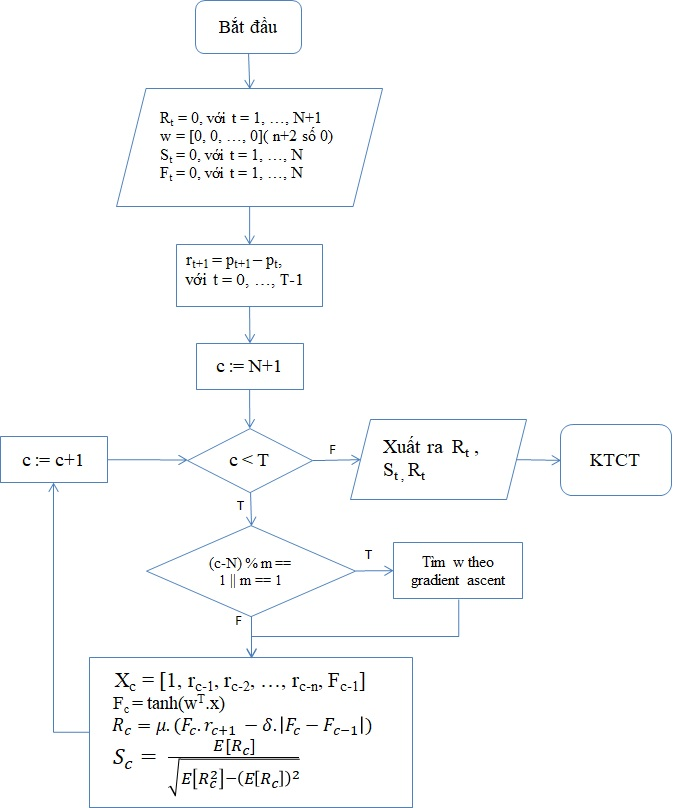
\includegraphics[scale=0.9]{Thuat_toan.jpg}
\end{center}

\chapter{Kết luận}

Dưới đây là một số kết quả khi chạy thuật toán để tìm ra phương án đầu tư cho mã cổ phiếu MSFT

\section{Liên tục cập nhập chiến lược càng nhiều thì khả năng cho lợi nhuận ổn định càng cao}

$\quad$Nhìn vào hình 4.1 và 4.2, ta có nhận xét rằng để chạy được ra kết quả hình 4.2 thì ta sẽ mất nhiều thời gian hơn( vì cứ 2 ngày ta lại phải luyện lại để tìm w) nhưng đồng thời cũng cho kết quả tốt hơn.

Vấn đề này không có gì là khó hiểu bởi lẽ, giá của cổ phiểu sẽ biến động theo một chu kì không dài vì nó thường xuyên ảnh hưởng bởi các yếu tố bên ngoài( chia cổ tức, công ty ra báo cáo tài chính).
\begin{center}
    \begin{figure}[htp]
    \begin{center}
     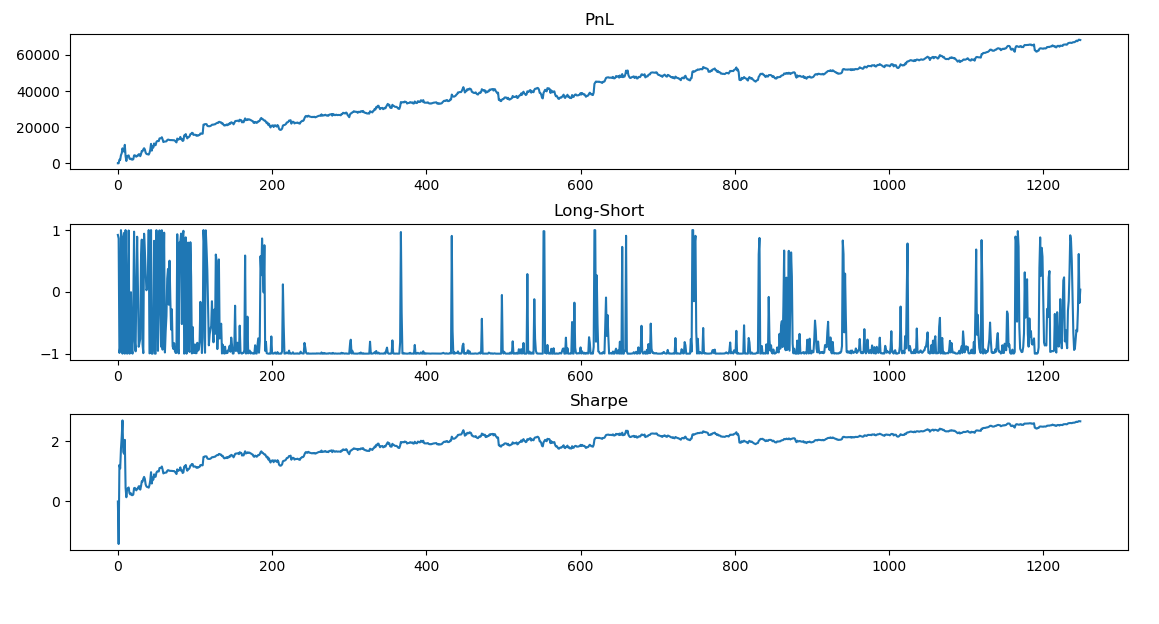
\includegraphics[scale=.4]{result_1-1}
    \end{center}
    \caption{T = 1280, n = 5, N = 30, m = 5}
    \begin{center}
     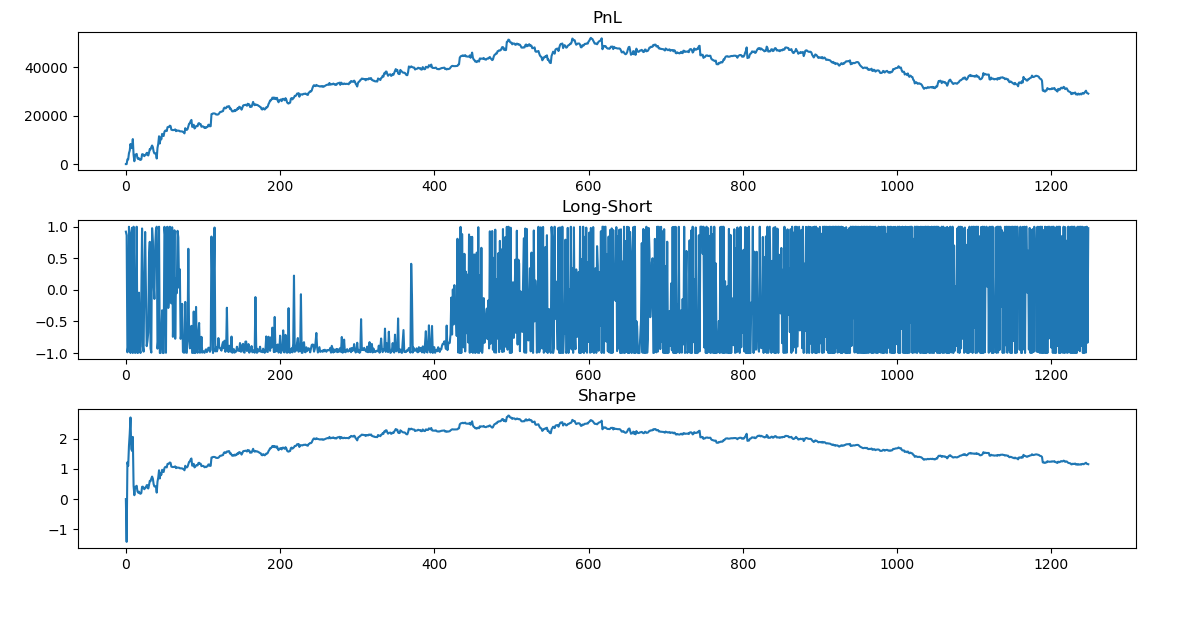
\includegraphics[scale=.4]{result_1-2}
    \end{center}
    \caption{T = 1280, n = 5, N = 30, m = 2}
    \end{figure}
\end{center} 

\newpage

Cũng vì lẽ chu kì này xảy ra ngắn nên nếu ta áp dụng một chiến thuật được xây dựng chưa cập nhập được xu thế của giá thì việc đầu tư sẽ khó mà gặp thuận lợi được.

Vì vậy, kết luận thứ nhất mà nhóm đưa ra là càng liên tục chiến thuật theo xu hướng của giá thì khả năng cho lợi nhuận ổn định càng cao.

Ngoài ra, ta có thể thấy việc chọn các giá trị n, N nên là bội của 5. Bởi lẽ, thị trường chứng khoán hoạt động 5 ngày/tuần nên việc sử dụng những con số này sẽ rất có ý nghĩa về mặt thực tế để tìm qui luật của giá chứng khoán.

\newpage

\section{Việc luyện nhiều bằng nhiều dữ liệu chưa hẳn đưa chiến lược w không tốt}

$\quad$Nhìn vào hình 4.3 và 4.4, ta có nhận xét rằng lợi nhuận trong hình 4.3 nhiều hơn không lại có sharpe thấp hơn

Việc này đi ngược với xu hướng chứng khoán thông thường vì giá cổ phiếu được thay đổi liên tục và không thể xảy ra trong thời gian dài được. 

Vì thế, ta thường luyện mô hình trong không quá dài. Tuy nhiên, việc này cũng không hẳn là đúng vì con số 60 cũng rất có ý nghĩa. Bởi lẽ, theo chu kì một quí( 60 ngày do thị trường chứng khoán hoạt động 5 ngày/ tuần) thì các công ti sẽ ra các báo cáo tài chính

Tóm lại, trong trường hợp này, kết luận của nhóm là không hẳn dữ liệu càng nhiều thì càng không cho mô hình tốt
\begin{center}
    \begin{figure}[htp]
    \begin{center}
     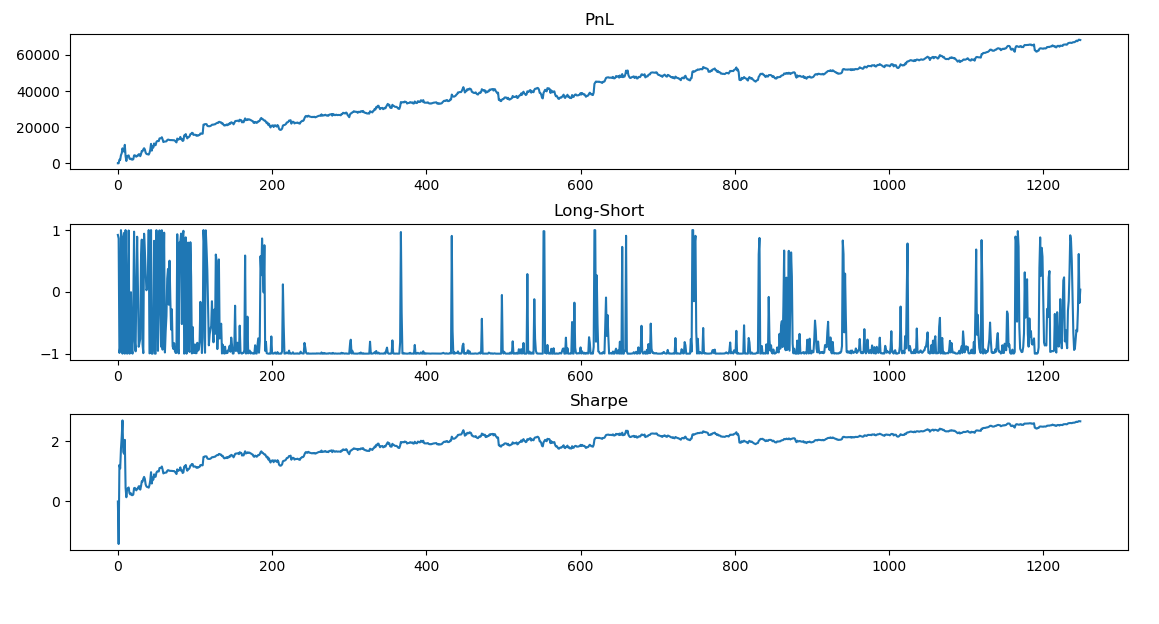
\includegraphics[scale=.4]{result_1-1}
    \end{center}
    \caption{T = 1280, n = 5, N = 30, m = 5}
    \begin{center}
     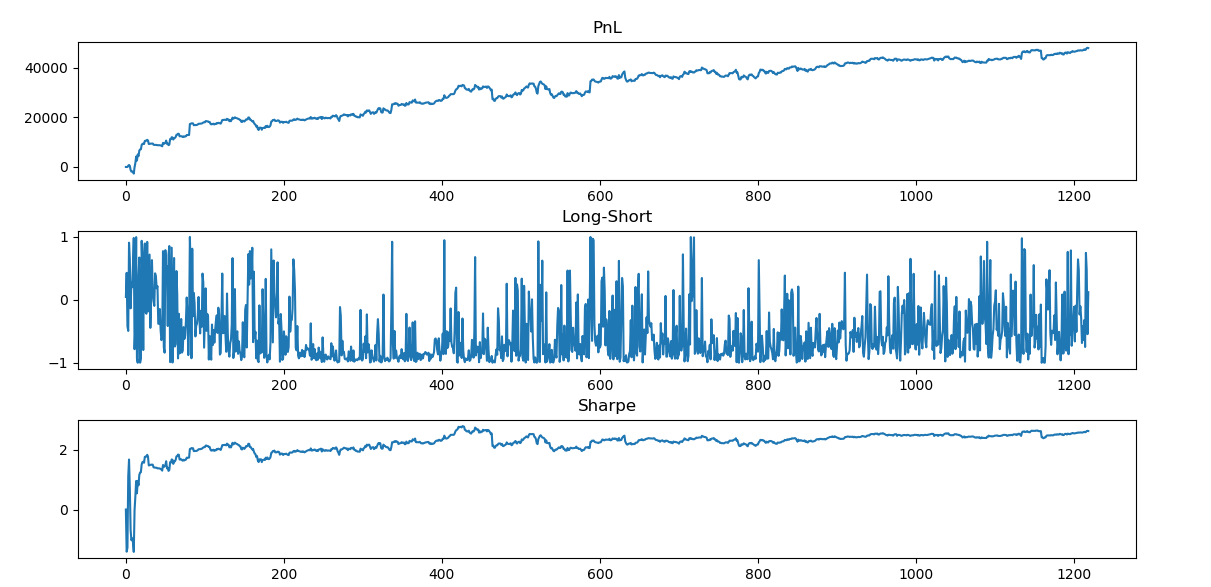
\includegraphics[scale=.4]{result_2-1}
    \end{center}
    \caption{T = 1280, n = 5, N = 60, m = 5}
    \end{figure}
\end{center} 

\addcontentsline{toc}{chapter}{{Danh mục công trình công bố của tác giả}}
\chapter*{Tiệu tham khảo}
\begin{flushleft}

\quad $[1]$\ Pierpaolo G. Necchi: \textit{ Reinforcement Learning For Automated Trading}

\quad $[2]$\ CS229 Application Project
Gabriel Molina, SUID 5055783: \textit{ Stock Trading with Recurrent Reinforcement
Learning (RRL)}
\end{flushleft}
\end{document}